\documentclass[20pt]{article}

\usepackage[a4paper]{geometry}
\usepackage{titlesec}
\usepackage{amsmath}
\usepackage{amssymb}
\usepackage{times}
\usepackage{tipa}
\usepackage{covington}
\usepackage{tikz}
\usepackage{tikz-qtree}

\setlength\parindent{0pt}
\newcommand{\ipa}[1]{\textipa{#1}}
\newcommand{\broad}[1]{/\ipa{#1}/}
\newcommand{\narrow}[1]{[ \ipa{#1} ]}
\newcommand{\english}[1]{$<$#1$>$}
\newcommand{\sk}[0]{{\kern 0.05em}}
\newcommand{\mk}[0]{{\kern 0.1em}}
\newcommand{\smallcapi}[0]{\sk\textsci\sk}
\newcommand{\openo}[0]{\sk O}

\titlespacing*{\section}{0pt}{0.7\baselineskip}{0.7\baselineskip}
\titleformat*{\section}{\large\bfseries}

\begin{document}

\Large\textbf{Problem Set 3} \\
\normalsize
Alice McKean \\
\today

\section{Phrase Structure Trees}

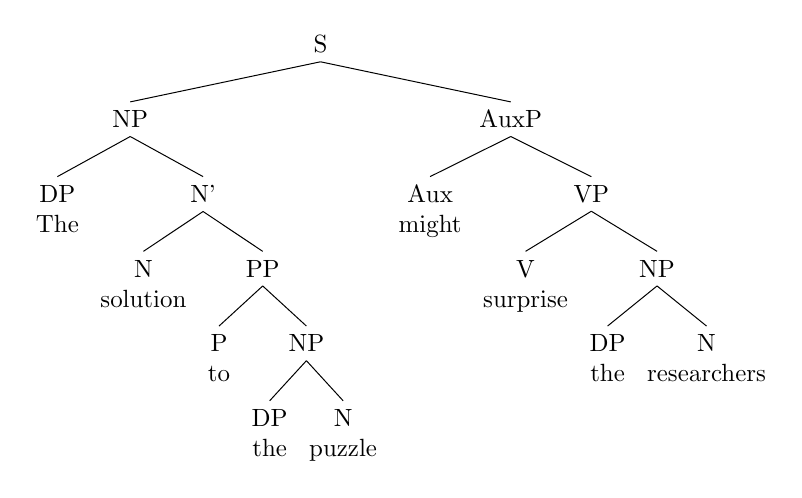
\begin{tikzpicture}[scale=0.9, transform shape]
  \tikzset{every tree node/.style={align=center,anchor=north}}
  \Tree [.S [.NP DP\\The
                 [.N' N\\solution
                      [.PP P\\to
                           [.NP DP\\the 
                                N\\puzzle
                           ]
                      ]
                 ]
            ]
            [.AuxP Aux\\might
                   [.VP V\\surprise
                        [.NP DP\\the 
                             N\\researchers
                        ]
                   ]
            ]
        ]
\end{tikzpicture}

\begin{tikzpicture}[scale=0.9, transform shape]
  \tikzset{every tree node/.style={align=center,anchor=north}}
  \Tree [.S NP\\They 
            [.VP AdvP\\soon
                 [.VP V\\discovered
                      [.CP C\\that 
                           [.S NP\\Dasha
                               [.VP [.VP V\\relies 
                                         [.PP P\\on
                                              NP\\me
                                         ]
                                    ]
                                    [.PP P\\for
                                         NP\\help
                                    ]
                               ]
                           ]
                      ]
                 ]
            ]
        ]
\end{tikzpicture}

\begin{tikzpicture}[scale=0.9, transform shape]
  \tikzset{every tree node/.style={align=center,anchor=north}}
  \Tree [.S NP\\Kai
            [.VP V\\disagreed
                 [.PP P\\with
                      [.NP DP\\that
                           [.N' AP\\negative
                                [.N' N\\review
                                     [.PP P\\of
                                          [.NP NP\\their
                                               [.N' AP\\favorite
                                                    N\\film
                                               ]
                                          ]
                                     ]
                                ]
                           ]
                      ]
                 ]
            ]
        ]
\end{tikzpicture}

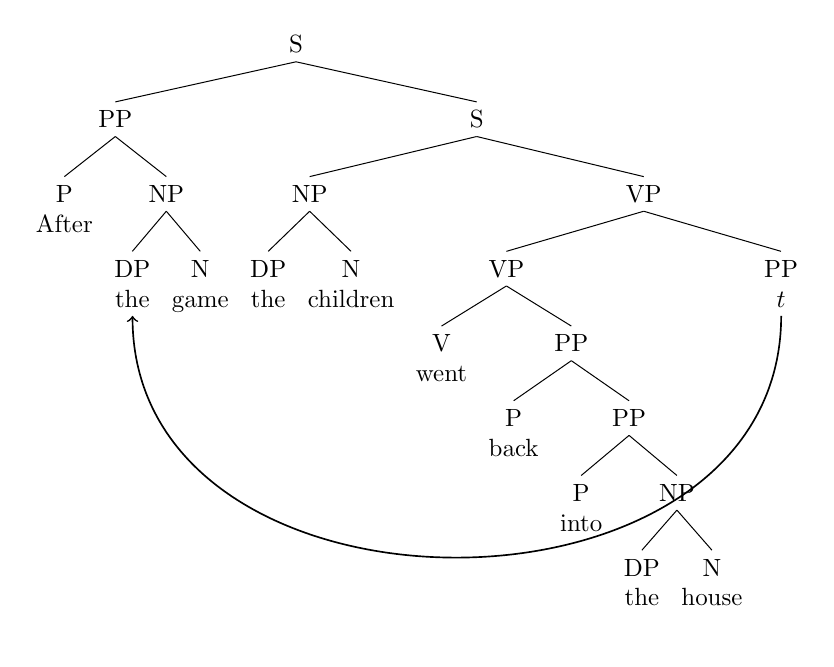
\begin{tikzpicture}[scale=0.9, transform shape]
  \tikzset{every tree node/.style={align=center,anchor=north}}
  \Tree [.S [.PP P\\After
                 [.NP \node(end){DP\\the}; N\\game ]
            ]
            [.S [.NP DP\\the N\\children ]
                [.VP [.VP V\\went
                          [.PP P\\back
                               [.PP P\\into
                                    [.NP DP\\the N\\house ]
                               ]
                          ]
                     ]
                     \node(start){PP\\$t$};
                ]
            ]
        ]
  \draw[semithick,->] (start)..controls +(south:5) and +(south:5)..(end);
\end{tikzpicture}

Back is a preposition as you can add right in front of it. The sentence ``After
the game, the children went right back into the house.'' is grammatical.
By the coordination test the substring ``went back into the house'' is a verb
phrase. This can be seen in the example sentence: ``After the game the children
went back into the house and slept''.
The substring ``into the house'' is a prepositional phrase as it can be replaced
by ``there''. The sentence ``After the game, the children went back
there'' is grammatical.
By a similar argument the substring ``back into the house'' is a prepositional
phrase as the sentence ``After the game the children went there'' is grammatical.
We haven't learned movement yet so I'm pretty sure I got it wrong but I wanted
to give it a try.

\section{Structural Ambiguity and Constituency}
Tree A: Wanda used a telescope to spy on the lemur. \\

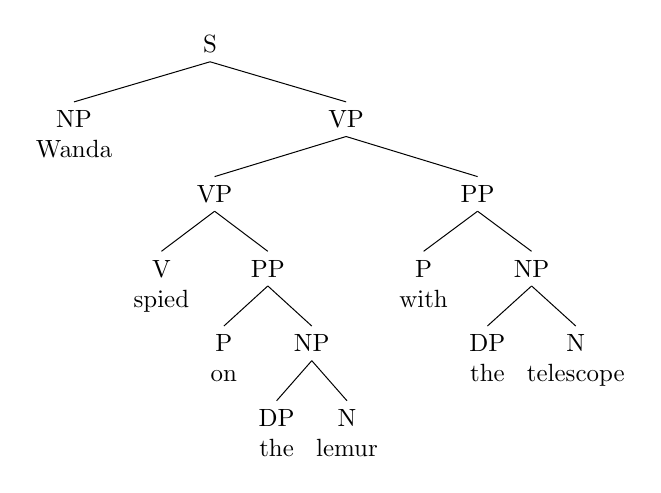
\begin{tikzpicture}[scale=0.9, transform shape]
  \tikzset{every tree node/.style={align=center,anchor=north}}
  \Tree [.S NP\\Wanda
            [.VP [.VP V\\spied 
                      [.PP P\\on 
                           [.NP DP\\the
                                N\\lemur
                           ]
                      ]
                 ]
                 [.PP P\\with
                      [.NP DP\\the N\\telescope ]
                 ]
            ]
        ]
\end{tikzpicture}

Tree B: Wanda spied on a lemur that has a telescope. \\

\begin{tikzpicture}[scale=0.9, transform shape]
  \tikzset{every tree node/.style={align=center,anchor=north}}
  \Tree [.S NP\\Wanda
            [.VP V\\spied
                 [.PP P\\on 
                      [.NP DP\\the
                           [.N' N\\lemur
                                [.PP P\\with
                                     [.NP DP\\the N\\telescope ]
                                ]
                           ]
                      ]
                 ]
            ]
        ]
\end{tikzpicture}

If you apply ``do so'' replacement to the inner VP in Tree A you get ``Wanda
did so with the telescope.'' If the lemur had the telescope what would Wanda
be doing? The top most PP can be fronted in Tree A to make it clear that Wanda
is using the Telescope: ``With the telescope Wanda spied on the lemur''.
The top most PP can be fronted in Tree B to make it clear that the
lemur has the telescope: ``On the lemur with the telescope Wanda spied''. You
can replace the main NP with a pronoun in Tree B: ``Wanda spied on it''. In this
sentence the lemur has to have the telescope because Wanda isn't using it to spy.

\end{document}

